% ====================================================
% SESSION 1 -- Why design at all?
% Body file, shared by introduction.tex and introduction_notes.tex
% ====================================================

% ----------------------------------------------------
\begin{frame}[plain]
  \titlepage
\end{frame}
% ----------------------------------------------------
\note{}

% ----------------------------------------------------
\begin{frame}
\frametitle{Introduction}
\centering

\begin{itemize}
  \item<1-> What is this course about?
  \item<1-> Expectations?
  \vspace{10pt}
  \item<2-> \textbf{What is research? And why do we need to design it?}
\end{itemize}

\end{frame}
% ----------------------------------------------------
\note{Open by asking them, not by answering. Two or three responses is enough. The point is to set the norm that this room talks.

Most will say something about ``methods'' or ``statistics''. Push back gently: this course has no statistics in it at all. What it has is the part that comes before, and the part that decides whether the statistics will mean anything.}

% ----------------------------------------------------
\begin{frame}
\frametitle{What this course is, and is not}
\centering

\vspace{5pt}
\begin{columns}[T]
\begin{column}{0.47\textwidth}
\centering \textbf{We do}
\vspace{4pt}
\hrule
\vspace{6pt}
\footnotesize
\begin{flushleft}
what variation a design exploits\\[4pt]
what has to be true for it to work\\[4pt]
how to tell whether an answer is any good
\end{flushleft}
\end{column}
\begin{column}{0.47\textwidth}
\centering \textbf{We don't}
\vspace{4pt}
\hrule
\vspace{6pt}
\footnotesize
\begin{flushleft}
estimation, models, statistics\\[4pt]
code, software, data wrangling\\[4pt]
\asher{$\rightarrow$ that is your methods sequence:\\statistics, causal inference,\\data science, R, data mining}
\end{flushleft}
\end{column}
\end{columns}

\vspace{18pt}
\uncover<2->{\footnotesize No statistics in this course at all. Not one equation.}

\end{frame}
% ----------------------------------------------------
\note{Put this up front, because it is the reasonable objection from a cohort who signed up for a \textit{computational} master's, and if you don't answer it in week 1 they will quietly wonder for five weeks.

The line that works: this programme already teaches you all of that, properly, in dedicated courses, some of which you are taking \textit{this semester}. What it does not teach anywhere else is the part that decides whether running the estimator was worth doing.

That framing matters. This is a division of labour, not a simplification: they have had basic statistics and they are not being protected from anything.

It also sets expectations for the essay: no analysis required, and none rewarded on its own.}

% ====================================================
\section{Why design at all?}
% ====================================================

% ----------------------------------------------------
\begin{frame}
\frametitle{A real example}
\centering

\begin{itemize}[<+->]
  \item Racing team deciding whether to race or not in the last session
  \item Car engine has blown out in 7 out of 24 past races
  \begin{itemize}
    \item Should we risk an explosion and go bankrupt or race?
  \end{itemize}
  \item A mechanic has a last-minute gut feeling that it might have to do with temperature (forecast for race: very cold day)
  \item Someone says: ``show me the data of the past failures!''
\end{itemize}

\end{frame}
% ----------------------------------------------------
\note{Do not reveal what this is yet. Let them work as the racing team.

Ask: you have the seven failures in front of you. What do you look at? Almost everyone will start reasoning about the seven failures: temperature at each one, whether it looks cold.

Hold that thought. The whole lesson is on the next slides.}

% ----------------------------------------------------
\begin{frame}[plain]
  \begin{tikzpicture}[remember picture, overlay]
    \node[at = (current page.center), yshift = 0cm] (cover) {%
      
\includegraphics[keepaspectratio, width=\paperwidth, height=\paperheight]{../img/challenger1}};
  \end{tikzpicture}
\end{frame}
% ----------------------------------------------------
\note{The seven failures, plotted against temperature. This is a reconstruction (Tufte's) of the evidence as it was considered the night before the launch, not the actual Thiokol chart.

Looks like no pattern. Temperature seems irrelevant. This is the chart that supported the decision to launch.}

% ----------------------------------------------------
\begin{frame}[plain]
  \begin{tikzpicture}[remember picture, overlay]
    \node[at = (current page.center), yshift = 0cm] (cover) {%
      
\includegraphics[keepaspectratio, width=\paperwidth, height=\paperheight]{../img/challenger2}};
  \end{tikzpicture}
\end{frame}
% ----------------------------------------------------
\note{Now with all 24 launches, the successes included. The pattern is obvious.

Say it plainly: \textbf{the answer was in the observations they didn't look at.} Nothing was wrong with the data, the statistics, or the people. The selection of which cases to examine was the whole ballgame.

This is selection on the dependent variable, and it is the single most common error in the theses you will write.}

% ----------------------------------------------------
\begin{frame}[plain]
  \begin{tikzpicture}[remember picture, overlay]
    \node[at = (current page.center), yshift = 0cm] (cover) {%
      
\includegraphics[keepaspectratio, width=\paperwidth, height=\paperheight]{../img/challenger_wiki}};
  \end{tikzpicture}
\end{frame}
% ----------------------------------------------------
\note{Reveal: Challenger, 28 January 1986. Seven people died. The O-ring failure was a temperature problem, and the engineers who worried about it could not make the case with the chart they had.

Worth saying: this is not a story about people being stupid. It is a story about a design error that looks completely reasonable from the inside.}

% ----------------------------------------------------
\begin{frame}
\frametitle{Challenger example}
\centering

\begin{itemize}
  \item \colorbox{yellow}{Explanatory} research
  \item What is the role of design here?
  \item<2-> Which observations to use
  \item<2-> What \textit{variation} we need to answer the question?
\end{itemize}

\end{frame}
% ----------------------------------------------------
\note{Name the two things design did here, because both come back every week:
\begin{itemize}
  \item \textbf{Which observations} enter the comparison
  \item \textbf{What variation} you need in order to see anything at all
\end{itemize}
With only failures, temperature does not vary in a usable way. You need launches that did \textit{not} fail to have a comparison.}

% ----------------------------------------------------
\begin{frame}[plain]
  \begin{tikzpicture}[remember picture, overlay]
    \node[at = (current page.center), yshift = 0cm] (cover) {%
      
\includegraphics[keepaspectratio, width=\paperwidth, height=.92\paperheight]{../img/plane_wwii}};
  \end{tikzpicture}
\end{frame}
% ----------------------------------------------------
\note{The same lesson in one picture. WWII bombers, returning from missions, with the bullet holes mapped. (The red-dot diagram is a modern illustration, not a wartime document, so don't let them cite it as one.)

Ask where they would add armour. Most say: where the dots are.

Wald's answer: armour where there are \textit{no} dots. The planes hit there did not come back, so they are not in your data. Same structure as Challenger: the informative observations are the missing ones.

Keep this image in mind; ``who is missing from this dataset?'' is a question you can ask about almost any found data source, and we will ask it again in week 2.}

% ----------------------------------------------------
\begin{frame}
\frametitle{Not only about data or empirical evidence}
\centering

\begin{itemize}
  \item The ``non-data'' part is also important:
  \item[] thinking about an answerable question, a coherent argument, and how to connect it to data
  \vspace{10pt}
  \item Also problematic because we all probably think we already know how it's done, but e.g. many final theses fail on this
\end{itemize}

\end{frame}
% ----------------------------------------------------
\note{This is the thesis statement of the course, so say it early and say it directly.

The things that break an MA thesis are almost never the estimator. They are: a question that cannot be answered, data of unknown provenance, and a measure that does not capture the concept. The estimators are covered properly elsewhere in this programme; here we do the part that decides whether any of that will be worth doing.}

% ----------------------------------------------------
\begin{frame}
\frametitle{Types of research}
\centering

\begin{itemize}
  \item \textit{Theoretical} and \colorbox{yellow}{\textit{empirical} research}
  \item<2-> \textit{Qualitative} and \colorbox{yellow}{\textit{quantitative} empirical research}
  \begin{itemize}
    \item<3-> Descriptive vs explanatory
  \end{itemize}
\end{itemize}

\end{frame}
% ----------------------------------------------------
\note{Locate the course: empirical, mostly quantitative. But note that nearly everything we cover applies to careful qualitative work too, since the logic of comparison does not change.

The descriptive/explanatory split at the bottom is a preview. We will expand it into three goals shortly.}

% ====================================================
\section{Three ways to answer a question}
% ====================================================

% ----------------------------------------------------
\begin{frame}
\frametitle{Three things you can do with data}
\centering

\begin{itemize}[<+->]
  \item \textbf{Describe}: what is the case? How much, where, for whom?
  \vspace{8pt}
  \item \textbf{Explain}: does $X$ cause $Y$, and through what?
  \vspace{8pt}
  \item \textbf{Predict}: given what I observe, what happens next, or elsewhere?
\end{itemize}

\end{frame}
% ----------------------------------------------------
\note{\textbf{This is the spine of the course.} Introduce it slowly and come back to it at the end of every session.

Three claims worth making explicitly:
\begin{itemize}
  \item They are different \textit{goals}, not difficulty levels. Description is not failed explanation.
  \item Each has its own success criteria, which is why the rest of the course exists.
  \item They get confused constantly, and that confusion is where most bad designs come from.
\end{itemize}
Also: this is the actual fault line in computational social science. You will hit it in every other course in this MA.}

% ----------------------------------------------------
\begin{frame}
\frametitle{Describe}
\centering


\includegraphics[keepaspectratio, width = 0.92\textwidth, height = 0.62\paperheight]{../img/facebook_separation}

\vspace{6pt}
{\footnotesize 1.59bn Facebook users; average degrees of separation $=3.57$.\\
No causal claim, no prediction, and still full of design decisions.}

\end{frame}
% ----------------------------------------------------
\note{``Six degrees of separation'', measured, on 1.59 billion Facebook users. The answer is about 3.57.

(Careful: the earlier 2012 study by Backstrom et al. used 721 million users and got 3.74. Different study, different number.)

Purely descriptive: no causal claim, no prediction. And yet full of design decisions: who counts as a user, what counts as a friendship, which population the average is over.

Chetty et al.'s social capital atlas (2022, \textit{Nature}) is the bigger version of the same idea: 21 billion Facebook friendships turned into a descriptive map of cross-class connectedness in the US. Mention it; we use it properly in week 3.}

% ----------------------------------------------------
\begin{frame}
\frametitle{Explain}
\centering


\includegraphics[keepaspectratio, width = 0.82\textwidth, height = 0.62\paperheight]{../img/guess2023}

\vspace{6pt}
{\footnotesize Feeds randomly switched from algorithmic to chronological, 3 months, $N\approx$ 23,000.\\
Randomisation buys the comparison. It does not buy generality.}

\end{frame}
% ----------------------------------------------------
\note{Guess et al. (2023), \textit{Science}. Facebook and Instagram feeds randomly switched from algorithmic ranking to reverse-chronological for three months during the 2020 US campaign.

This is your week-4 paper, so plant it now. The design question: what does randomisation buy you, and what does it still not buy you?

Answer to hold back until week 4: it buys you the comparison, and it does not buy you generality: one platform, one campaign, three months.}

% ----------------------------------------------------
\begin{frame}
\frametitle{Predict}
\centering


\includegraphics[keepaspectratio, width = 0.92\textwidth, height = 0.62\paperheight]{../img/blumenstock}

\vspace{6pt}
{\footnotesize Phone metadata $\rightarrow$ wealth estimates for a whole country.\\
Identifies nothing causal, and does not need to. It has to work \textit{out of sample}.}

\end{frame}
% ----------------------------------------------------
\note{Blumenstock, Cadamuro \& On (2015), \textit{Science}. Phone metadata (who called whom, when, for how long) used to estimate wealth across Rwanda, where reliable and frequent wealth data barely exists.

The key point, and the reason prediction is in this course: this design does not identify anything causal, and it does not need to. It has to work out of sample. That is a completely different standard of success.

If a student's project is really a prediction problem, holding it to causal standards will make it worse, not better.}

% ----------------------------------------------------
\begin{frame}
\frametitle{Different goals, different standards}
\centering

\vspace{5pt}
\footnotesize
\begin{tabularx}{\textwidth}{p{2.1cm}|L|L}
\textbf{Goal} & \textbf{Succeeds when} & \textbf{Typical failure} \\
\hline
\textbf{Describe} & coverage, comparability, a defensible denominator & measuring what got recorded, not what happened \\
\hline
\textbf{Explain} & the comparison isolates the effect & something else moved at the same time \\
\hline
\textbf{Predict} & it works out of sample & it worked, until the world changed \\
\end{tabularx}

\vspace{12pt}
\begin{itemize}
  \item<2-> Most bad designs are a \textbf{mismatch}: a descriptive question with a causal answer bolted on, or a causal question answered with a predictive design
\end{itemize}

\end{frame}
% ----------------------------------------------------
\note{The table is the payoff of the triad, and it is why naming the goal is not just terminology.

The mismatch line is the practical one. In the workshop you will diagnose half the projects in the room with exactly that sentence, so it is worth them hearing it in week 1.

Each row also previews a session: describe $\rightarrow$ week 3, explain $\rightarrow$ week 4, predict $\rightarrow$ closing of week 5.}

% ----------------------------------------------------
\begin{frame}
\frametitle{The five questions of this course}
\centering

\vspace{5pt}
\small
\begin{enumerate}
  \item \textbf{Why design at all?} \hfill \asher{today}
  \vspace{6pt}
  \item \textbf{What is the question, and where would the data come from?}
  \vspace{6pt}
  \item \textbf{Do the numbers mean what you think they mean?}
  \vspace{6pt}
  \item \textbf{What comparisons can we use to establish causal claims?}
  \vspace{6pt}
  \item \textbf{What variation can you exploit, and how far does the answer travel?}
\end{enumerate}

\vspace{10pt}
\begin{flushleft}
\footnotesize By the workshop, you should be able to answer all five \textit{about your own project}.
\end{flushleft}

\end{frame}
% ----------------------------------------------------
\note{The course map. It comes back at the start of every session with the current question highlighted. One slide a week, and it is what makes five lectures feel like one argument rather than a list of topics.

Say the last line out loud. The five questions are also the five memos, and the memos assemble into the essay. Nothing in this course is busywork bolted onto the assessment.}

% ====================================================
\section{Evidence, claims, and inference}
% ====================================================

% ----------------------------------------------------
\begin{frame}
\frametitle{Empirical research}
\centering

\begin{itemize}
  \item Goal: answer a question using empirical evidence
  \begin{itemize}
    \item Usual problems: unanswerable questions, wrong data to question, concepts do not correspond to measurements...
  \end{itemize}
  \item<2-> How? exploiting \textbf{empirical variation}
  \item<2-> Research design is essentially knowing where to look at, how to measure it, how to analyze it, how to interpret it, etc --
  \item[] it's about \colorbox{yellow}{inference}
  \item[] {\footnotesize \asher{using what you \textit{did} observe to say something about what you did \textit{not}}}
  \item<3-> Two things we should learn:
  \item[] how to answer questions \& how to evaluate answers
\end{itemize}

\end{frame}
% ----------------------------------------------------
% NOTE TO SELF: merged from two near-identical slides in the old deck.
\note{The second half matters as much as the first: half of what this course is for is making you a better \textit{reader}. Most of you will evaluate far more research than you produce.}

% ----------------------------------------------------
\begin{frame}
\frametitle{Empirical evidence and claims}
\centering


\includegraphics[keepaspectratio, width = 0.65\textwidth, height = 0.78\paperheight]{../img/nyt_museums}

\end{frame}
% ----------------------------------------------------
\note{Let them read it. Then: what would you have had to do to be able to write this headline?}

% ----------------------------------------------------
\begin{frame}
\frametitle{Empirical evidence and claims}
\centering

\begin{itemize}
  \item Let's reverse-engineer this:
  \begin{itemize}
    \item What did they probably do?
  \end{itemize}
  \item How would you answer the question better?
  \item<2-> Causal inference and experimental methods
  \begin{itemize}
    \item Observation vs manipulation
  \end{itemize}
  \item<3-> Gold standard?
\end{itemize}

\end{frame}
% ----------------------------------------------------
\note{Reverse-engineering a headline is a skill worth practising, and they will do it again in the audit exercise later today.

Get to the observation/manipulation distinction, and then put a question mark on ``gold standard''. Experiments are not automatically better; they are better at one specific thing. We return to this in week 4.}

% ----------------------------------------------------
\begin{frame}[plain]
  \begin{tikzpicture}[remember picture, overlay]
    \node[at = (current page.center), yshift = 0cm] (cover) {%
      
\includegraphics[keepaspectratio, width=\paperwidth, height=\paperheight]{../img/psycho1}};
  \end{tikzpicture}
\end{frame}
% ----------------------------------------------------
\note{A widely reported psychology finding, presented at face value. Let them read it and react before you say anything, because the reaction is the material.}

% ----------------------------------------------------
\begin{frame}
\frametitle{Opinions about claims?}
\centering


\includegraphics[width = \textwidth]{../img/psycho4}

\end{frame}
% ----------------------------------------------------
\note{Push them to separate two different objections: ``I don't believe the finding'' and ``I don't believe the design could have found that''. Only the second is a research design objection, and it is the one worth learning to make.}



% ----------------------------------------------------
\begin{frame}[plain]
  \begin{tikzpicture}[remember picture, overlay]
    \node[at = (current page.center), yshift = 0cm] (cover) {%
      
\includegraphics[keepaspectratio, width=\paperwidth, height=\paperheight]{../img/marshmallow}};
  \end{tikzpicture}
\end{frame}
% ----------------------------------------------------
\note{The marshmallow test: children who wait for a second marshmallow do better in life. Famous, endlessly repeated in popular writing.}

% ----------------------------------------------------
\begin{frame}[plain]
  \begin{tikzpicture}[remember picture, overlay]
    \node[at = (current page.center), yshift = 0cm] (cover) {%
      
\includegraphics[keepaspectratio, width=\paperwidth, height=\paperheight]{../img/marshmallow3}};
  \end{tikzpicture}
\end{frame}
% ----------------------------------------------------
\note{And the replication (Watts, Duncan \& Quan 2018), with a larger and more diverse sample: the association is \textit{largely attenuated} once family background is accounted for. Not eliminated, but much smaller than the famous version.

The design lesson: the original comparison was between children who differed in a great many ways besides willpower. Same data pattern, entirely different explanation, and you cannot tell which from the correlation alone. That gap is what weeks 4 and 5 are about.}

% ----------------------------------------------------
\begin{frame}
\frametitle{Other types of inference}
\centering

\begin{itemize}
  \item We are used to cases where we compare many observations with different values on key variables
  \item What if we don't have enough observations to answer a question?
  \item Any idea about examples?
\end{itemize}

\end{frame}
% ----------------------------------------------------
\note{Let them try. Usual answers: rare events, single countries, historical cases, one-off disasters.

The point is not that these are impossible, but that they need a different kind of design: the variation has to come from somewhere other than ``lots of units''.}

% ----------------------------------------------------
\begin{frame}[plain]
  \begin{tikzpicture}[remember picture, overlay]
    \node[at = (current page.center), yshift = 0cm] (cover) {%
      
\includegraphics[keepaspectratio, width=\paperwidth, height=\paperheight]{../img/derecho2022a}};
  \end{tikzpicture}
\end{frame}
% ----------------------------------------------------
\note{A press report attributing a specific extreme weather event to climate change. Ask how anyone could possibly know that, given there is only one of this event.}

% ----------------------------------------------------
\begin{frame}
\frametitle{Opinions? How do you think it's done?}
\centering


\includegraphics[width = \textwidth]{../img/derecho2022c}

\end{frame}
% ----------------------------------------------------
\note{Attribution science: how can anyone say a specific heatwave was made more likely by climate change, when there is only one heatwave?

Let them speculate before revealing. The answer (simulate the world with and without) is a preview of potential outcomes in week 4, and it is worth flagging as such.}

% ----------------------------------------------------
\begin{frame}[plain]
  \begin{tikzpicture}[remember picture, overlay]
    \node[at = (current page.center), yshift = 0cm] (cover) {%
      
\includegraphics[keepaspectratio, width=\paperwidth, height=\paperheight]{../img/derecho2022b}};
  \end{tikzpicture}
\end{frame}
% ----------------------------------------------------
\note{The variation is generated by the model, not observed in the world. That is a legitimate design, and it makes the assumptions completely explicit, which is more than can be said for a lot of observational work.}

% ----------------------------------------------------
\begin{frame}<1>[label=variation]
\frametitle{A few questions on variation}
\centering

\begin{itemize}
  \item Why do we talk so much about \textit{variation}?
  \item<2-> Critique of having ``few observations''?
  \item<3-> Why do we use statistics at all?
  \item<4-> What about experiments?
  \item<5-> Where's the variation in attribution science?
\end{itemize}

\end{frame}
% ----------------------------------------------------
\note{Socratic block. Go slowly, one at a time, and let silences sit. This is the highest-value twenty minutes of the first hour.

Take only the first question now; the slide comes back after the eclipse image.}

% ----------------------------------------------------
\begin{frame}[plain]
  \begin{tikzpicture}[remember picture, overlay]
    \node[at = (current page.center), yshift = 0cm] (cover) {%
      
\includegraphics[keepaspectratio, width=\paperwidth, height=\paperheight]{../img/halley_eclipse}};
  \end{tikzpicture}
\end{frame}
% ----------------------------------------------------
\note{Halley's eclipse map. One prediction, no sample, no statistics, and a genuinely strong test, because the theory said exactly where the shadow would fall and it fell there.

Use it against the reflex that ``more observations = better evidence''. What makes evidence strong is how much it could have gone the other way.}

% ----------------------------------------------------
\againframe<2->{variation}
% ----------------------------------------------------
\note{Now work through the rest.

\begin{itemize}
  \item \textbf{Few observations:} not fatal in itself. The question is whether the comparison is informative.
  \item \textbf{Why statistics:} to separate signal from noise, not to create knowledge. Statistics answers ``could this be chance?'', never ``does this design identify anything?''
  \item \textbf{Experiments:} they manufacture the variation instead of waiting for it.
  \item \textbf{Attribution science:} the variation is simulated.
\end{itemize}}

% ----------------------------------------------------
\begin{frame}
\frametitle{Description is not easy either}
\centering

\begin{itemize}
  \item Are levels of political violence increasing?
  \item<2-> Is the world becoming less democratic?
\end{itemize}

\end{frame}
% ----------------------------------------------------
\note{Both sound like simple lookups. Neither is.

Push on the first: increasing compared to when? counting what: deaths, events, participants? per capita or absolute? recorded by whom, and has recording itself changed?

Do not resolve it. This is the trailer for week 3, where description gets a full session.}

% ====================================================
\section{Units, observations, variation}
% ====================================================

% ----------------------------------------------------
\begin{frame}
\frametitle{Key ingredients}
\centering

\vspace{2pt}
{\footnotesize A dataset, and the four words we will use every week:}

\vspace{6pt}
\begin{tikzpicture}[font=\footnotesize]
  \matrix (m) [matrix of nodes, ampersand replacement=\&, nodes={draw=asher!40, minimum width=2.1cm, minimum height=0.52cm, anchor=center},
               row sep=-\pgflinewidth, column sep=-\pgflinewidth,
               row 1/.style={nodes={fill=asher!15, font=\footnotesize\bfseries}}]
  {
    country \& year  \& GDP p/c \\
    Spain   \& 2020  \& 27{,}100 \\
    Spain   \& 2021  \& 30{,}100 \\
    France  \& 2020  \& 39{,}000 \\
    France  \& 2021  \& 43{,}700 \\
  };
  \draw[accent2, thick] (m-3-1.north west) rectangle (m-3-3.south east);
  \node[accent2, right = 4pt of m-3-3, font=\footnotesize] {one \textbf{observation}};
  \draw[accent, thick] (m-1-3.north west) rectangle (m-5-3.south east);
  \node[accent, below = 3pt of m-5-3, font=\footnotesize] {a \textbf{variable}};
  \node[asher, left = 4pt of m-1-1, font=\footnotesize, align=right] {\textbf{unit of}\\\textbf{analysis:}\\country-year};
\end{tikzpicture}

\vspace{8pt}
{\footnotesize \textbf{Variation} $=$ the differences \textit{down} a column that a comparison can use.\\
No variation, nothing to learn.}

\end{frame}
% ----------------------------------------------------
\note{Replaces a bare list of four nouns. Walk the picture slowly, since it is the only formal thing in the whole session, and every later week refers back to it.

\begin{itemize}
  \item \textbf{Observation}: one row.
  \item \textbf{Unit of analysis}: what a row \textit{is}. Here country-year, not country: Spain appears twice.
  \item \textbf{Variable}: one column.
  \item \textbf{Variation}: the spread down a column.
\end{itemize}

The last line is the one that matters, and it is the Challenger lesson restated: with only failures, the outcome column does not vary, so no comparison is available. Worth saying that explicitly --- it links the vocabulary back to the opening.}

% ----------------------------------------------------
\begin{frame}
\frametitle{On the unit of analysis}
\centering

\begin{itemize}
  \item Why is this important?
  \item<2-> Able to quickly identify it?
\end{itemize}

\end{frame}
% ----------------------------------------------------
\note{Being able to name the unit of analysis in five seconds, from a graph or an abstract, is a genuinely useful reflex. Next three slides are practice.}

% ----------------------------------------------------
\begin{frame}
\frametitle{What's the unit of analyses in the data behind this graph?}
\centering


\includegraphics[width = 0.8\textwidth]{../img/ua1}

\end{frame}
% ----------------------------------------------------
\note{\textbf{Answer:} the country, in a single year (2006). Press on whether that makes it country or country-year. With one year there is no time variation, so it is a cross-section.

Make them commit to an answer before you reveal it.}

% ----------------------------------------------------
\begin{frame}[plain]
  \begin{tikzpicture}[remember picture, overlay]
    \node[at = (current page.center), yshift = 0cm] (cover) {%
      
\includegraphics[keepaspectratio, width=\paperwidth, height=\paperheight]{../img/ua2}};
  \end{tikzpicture}
\end{frame}
% ----------------------------------------------------
\note{\textbf{Read this one out, it is in Spanish.} \textit{Median income per living unit, by family type and autonomous community} (INE/El Pa\'is): green = all households, orange = large families, red = one adult with 1--2 dependent children.

\textbf{Answer:} the unit is the surveyed \textit{household}, displayed aggregated to region $\times$ family type.

And read the footnote out too, because it is the best thing on the slide: \textit{``the data for Extremadura, Arag\'on, Canarias, Cantabria, La Rioja and Asturias are based on only 50 to 100 interviews.''} Six of the eighteen regions are estimated off almost nothing, and the chart gives every dot the same visual weight.}

% ----------------------------------------------------
\begin{frame}[plain]
  \begin{tikzpicture}[remember picture, overlay]
    \node[at = (current page.center), yshift = 0cm] (cover) {%
      
\includegraphics[keepaspectratio, width=\paperwidth, height=\paperheight]{../img/ua3}};
  \end{tikzpicture}
\end{frame}
% ----------------------------------------------------
\note{\textbf{Answer:} the individual award-winner, displayed as a smoothed (12-year moving average) series by category and year.

Note how often the graph shows one unit while the data underneath is at another, aggregated up for display. That gap has a name, the \textbf{ecological fallacy}: what holds for regions need not hold for the people in them. Say it once here; it comes back whenever they aggregate.}

% ----------------------------------------------------
\begin{frame}
\frametitle{On the unit of analysis}
\centering

\begin{itemize}
  \item Most empirical designs can be adapted to different units of analyses
  \item The unit you use is related to the question and theory
  \item<2-> Example: children's educational attainment and contextual factors (peers, school, family, etc)
  \begin{itemize}
    \item<2-> How many different units could you use, and how do they map onto different questions?
  \end{itemize}
\end{itemize}

\end{frame}
% ----------------------------------------------------
\note{Child, classroom, school, neighbourhood, cohort: each is a different question, not a different way of asking the same one.

This sets up the hotel booking thesis later in the session, where a badly chosen unit quietly changes what is being asked.}

% ====================================================
\section{From data to a question}
% ====================================================

% ----------------------------------------------------
\begin{frame}
\frametitle{Where does your data come from?}
\centering

\vspace{5pt}
\begin{columns}[T]
\begin{column}{0.47\textwidth}
\centering \textbf{Designed}
\vspace{4pt}
\hrule
\vspace{6pt}
\footnotesize
surveys, experiments,\\a coding scheme you wrote
\vspace{8pt}
\begin{flushleft}
$\rightarrow$ answers a question \textbf{you} had
\end{flushleft}
\end{column}
\begin{column}{0.47\textwidth}
\centering \textbf{Found}
\vspace{4pt}
\hrule
\vspace{6pt}
\footnotesize
digital traces, admin records,\\scraped text, API dumps
\vspace{8pt}
\begin{flushleft}
$\rightarrow$ answers a question \textbf{someone else} had.\\Or no question at all
\end{flushleft}
\end{column}
\end{columns}

\vspace{18pt}
\uncover<2->{Almost everything you will work with in this MA is \colorbox{yellow}{found data}}

\end{frame}
% ----------------------------------------------------
\note{One frame now, a full block next week, but plant the distinction here because the two theses coming up are both found data, and so is almost every project they will propose.

The sentence to land: found data was produced by someone, for their own purposes, and those purposes are still in the data. Facebook did not build a friendship graph so you could measure social capital.}

% ----------------------------------------------------
\begin{frame}
\frametitle{Two theses from this programme}
\centering

\vspace{10pt}
\begin{flushleft}
Both started the way most of yours will start: \textbf{with data already in hand}, and no question yet.
\end{flushleft}

\vspace{15pt}
\begin{itemize}
  \item<2-> A hotel's booking records
  \item<2-> Spotify's collaboration network
\end{itemize}

\end{frame}
% ----------------------------------------------------
\note{These are real TFMs from this master's, \textbf{anonymised and used with permission}. Say both halves, and say them unprompted. These students will hand in five memos and a design of their own, and how you treat other people's student work is how they will assume theirs gets treated.

Saying they are real changes how they listen.

Starting from data rather than from a question is not a sin, and pretending otherwise would be dishonest. It is just the harder direction to work in, and it needs the discipline this course teaches.}

% ----------------------------------------------------
\begin{frame}
\frametitle{Thesis 1: hotel bookings}
\centering

\begin{itemize}[<+->]
  \item Data arrives from a hotel: every booking, and whether the guest actually showed up
  \item Unit of analysis: \textbf{the booking}
  \vspace{12pt}
  \item \textbf{Motivation:} ``how do we increase business for the hotel?''
  \vspace{6pt}
  \item \textbf{Research question:} \makebox[3.5cm]{\hrulefill}\,?
\end{itemize}

\end{frame}
% ----------------------------------------------------
\note{Leave the blank on screen and let it sit.

``How do we increase business for the hotel?'' is a perfectly good \textbf{motivation}: it says why anyone should care, and it is why the data exists at all. It is not a research question. Nothing about it tells you what to compare with what.

That gap is the single most common problem in a first thesis draft, and we name it explicitly in a few slides (``motivation is not a question''). Here they get to feel it before it has a label.

Do not mock the original. Almost every first draft starts exactly here.}

% ----------------------------------------------------
\begin{frame}
\frametitle{Thesis 1: what can these data answer?}
\centering

\begin{itemize}[<+->]
  \item Which \textbf{goal} could this be: describe, explain, or predict?
  \item What would each version actually look like?
  \item Is ``the booking'' the right \textbf{unit}? What else could it be?
  \item Who is \textbf{missing} from this data?
  \vspace{8pt}
  \item And: is the question you can answer the one the hotel wanted?
\end{itemize}

\end{frame}
% ----------------------------------------------------
\note{Work it live. The framing: motivation fixed, data fixed. Now what question is actually available?

{\footnotesize
\begin{itemize}
  \item \textbf{Describe:} what share of bookings are no-shows, and how does that vary by season, channel, price?
  \item \textbf{Explain:} does requiring a deposit reduce no-shows? Needs a comparison, and the hotel changed its policy for a reason.
  \item \textbf{Predict:} flag likely no-shows so rooms can be resold. Fine, and needs no causal claim at all.
\end{itemize}}

Unit: booking, guest, room-night, season. A repeat guest with ten bookings is ten observations --- is that what you want? Missing: people who wanted to book and couldn't. Callback to the bombers.

\textbf{Last bullet is the payoff.} The hotel wanted more business; what the data supports is mostly a no-show question. Noticing that gap --- rather than answering the easier question and presenting it as the harder one --- is the skill.}

% ----------------------------------------------------
\begin{frame}
\frametitle{Thesis 2: music collaborations}
\centering


\includegraphics[width = 0.9\textwidth]{../img/spotify}

\vspace{8pt}
\begin{itemize}
  \item Spotify API data, turned into a \textbf{network} of artist collaborations
  \item Variables available: time, genre
\end{itemize}

\end{frame}
% ----------------------------------------------------
\note{Data pulled from the API, reshaped into a network: artists as nodes, a shared track as an edge.

Genuinely interesting data. But note what happened: the structure of the analysis (a network) was decided before the question was.}

% ----------------------------------------------------
\begin{frame}
\frametitle{Thesis 2: what can we ask here?}
\centering

\begin{itemize}[<+->]
  \item Is the unit the \textbf{artist}, the \textbf{collaboration}, or the \textbf{genre}?
  \item Are genres becoming more connected over time, or is Spotify's catalogue just growing?
  \item Who decides what counts as a ``genre'' here?
  \item If the platform changes how it tags artists, what happens to your trend?
\end{itemize}

\end{frame}
% ----------------------------------------------------
\note{The second and fourth questions are the important ones, and they are the same question in two forms: \textbf{is this a fact about music, or a fact about Spotify?}

Genre labels are Spotify's, produced for recommendation, not for research. If they retag, the measured trend moves without anything happening in the world.

This is exactly the Google Flu problem, which is next week's paper. Say so --- it makes the reading feel like it was assigned for a reason.}

% ----------------------------------------------------
\begin{frame}
\frametitle{What both have in common}
\centering

\vspace{15pt}
\begin{itemize}[<+->]
  \item Both are \textbf{found} data
  \item Both entered the process \textbf{in the middle} (at the data, not at the question)
  \vspace{10pt}
  \item Neither dataset came with a \textbf{goal}, a \textbf{unit}, or a \textbf{question}
\end{itemize}

\vspace{20pt}
\uncover<4->{\centering That is what the rest of this course supplies.}

\end{frame}
% ----------------------------------------------------
\note{The takeaway that both examples were building to, and the bridge into the research-process diagram.

Do not let them conclude that starting from data is illegitimate. Most of them will do it, and much good research does. The point is that the goal, the unit and the question then have to be supplied deliberately, by them, rather than inherited from whoever built the dataset.}

% ----------------------------------------------------
\begin{frame}
\frametitle{The research process}
\centering

\resizebox{\linewidth}{!}{
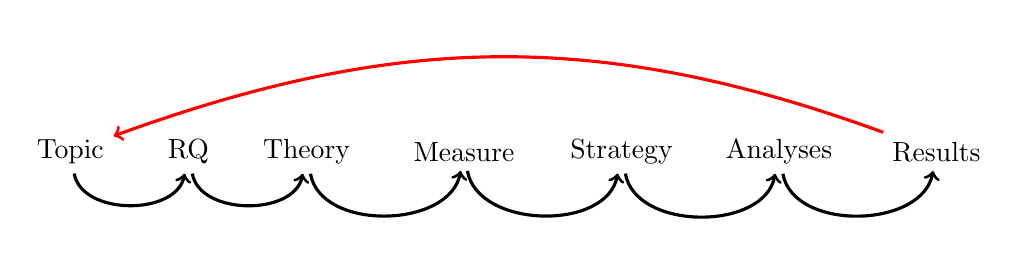
\begin{tikzpicture}
\node (topic) at (1,0) {Topic};
\node (rq) at (2.5,0) {RQ};
\node (theory) at (4,0) {Theory};
\node (measure) at (6,0) {Measure};
\node (strat) at (8,0) {Strategy};
\node (analyses) at (10,0) {Analyses};
\node (results) at (12,0) {Results};

\draw[->, line width=0.4mm] (topic) to[out=280, in=260] (rq) node[] {};
\draw[->, line width=0.4mm] (rq) to[out=280, in=260] (theory) node[] {};
\draw[->, line width=0.4mm] (theory) to[out=280, in=260] (measure) node[] {};
\draw[->, line width=0.4mm] (measure) to[out=280, in=260] (strat) node[] {};
\draw[->, line width=0.4mm] (strat) to[out=280, in=260] (analyses) node[] {};
\draw[->, line width=0.4mm] (analyses) to[out=280, in=260] (results) node[] {};
\draw[->, line width=0.4mm, red] (results) to[out=160, in=20] (topic) node[] {};

\end{tikzpicture}}

\vspace{20pt}
\begin{flushleft}
\footnotesize The red arrow is the honest part: nobody does this once, in order.
\end{flushleft}

\end{frame}
% ----------------------------------------------------
\note{The textbook version. Worth showing, worth immediately qualifying.

Both theses we just discussed entered this diagram in the middle (at ``Measure'') and had to work backwards to the question. That is normal, and the diagram does not show it.}

% ----------------------------------------------------
\begin{frame}
\frametitle{From topic to question, and from question to theory}
\centering

\begin{itemize}
  \item[$>$] From \textbf{topic} to the \BGyellow{\textbf{research question}}
  \begin{itemize}
    \item Motivation is not a question
    \item Good ones are answerable and relevant
  \end{itemize}
  \vspace{8pt}
  \item<2->[$>$] Examples, good and bad:
  \begin{itemize}
    \item<2-> What is the best Netflix show?
    \item<2-> What can we do to help poor countries develop?
    \item<2-> What are the shopping patterns of the Spanish population?
    \item<2-> Do individuals from minorities support the use of violence?
  \end{itemize}
  \vspace{8pt}
  \item<3->[$>$] From \textbf{RQ} to \BGyellow{\textbf{theory}}: arguments and mechanisms, testable and credible
\end{itemize}

\end{frame}
% ----------------------------------------------------
% NOTE TO SELF: compressed from six slides to two.
\note{In week 1 they have nothing to hang the detail on, and all of it returns properly in week 2.

Run the four examples quickly as a group: which are answerable, which are questions at all? The third is answerable but descriptive and vague; the fourth is answerable but needs a lot of conceptual work before it means anything.}

% ----------------------------------------------------
\begin{frame}
\frametitle{And the rest of the process}
\centering

\begin{itemize}
  \item[$>$] From \textbf{theory} to \BGyellow{\textbf{measurement}}: concepts, operationalization, unit of analysis \hfill \asher{(week 3)}
  \vspace{8pt}
  \item[$>$] From \textbf{measurement} to \BGyellow{\textbf{strategy}}: what variation will you look at? \hfill \asher{(weeks 4--5)}
  \vspace{8pt}
  \item[$>$] From \textbf{strategy} to \textbf{analyses}: \textit{not covered in this course}
  \begin{itemize}
    \item \textbf{Question:} what is the role of statistics in research design?
  \end{itemize}
  \vspace{8pt}
  \item[$>$] From \textbf{analyses} to \textbf{results}: interpretation, relevance, \textbf{external validity}
\end{itemize}

\end{frame}
% ----------------------------------------------------
\note{The week numbers on the right are deliberate: they tell them the course has a shape.

Do spend a minute on the statistics question. The answer worth giving: statistics tells you whether a pattern could be chance. It cannot tell you whether the comparison you made was the right one. A perfectly executed regression on a badly designed comparison is a precise answer to the wrong question.}

% ----------------------------------------------------
\begin{frame}
\frametitle{Simplifying}
\centering

\begin{itemize}
  \item[1.] Formulate one (or more) RQ from a topic/problem
  \item[2.] Develop a theoretical argument related to that RQ
  \item[3.] Building on theory, think about what and how to measure
  \item[4.] What variation are you going to look at?
  \item[5.] What can you really learn from the results?
\end{itemize}

\end{frame}
% ----------------------------------------------------
\note{The version to remember. It is also, more or less, the structure of the final essay. Point that out.}

% ====================================================
\section{Exercise: audit a claim}
% ====================================================

% ----------------------------------------------------
\begin{frame}
\frametitle{Exercise: audit a claim}
\centering

\vspace{2pt}
\begin{itemize}
  \item[\textbf{A.}] ``Remote work has made young people lonelier.''
  \item[\textbf{B.}] ``Four in ten Spanish adults under 30 still live with their parents.''
  \item[\textbf{C.}] ``Our model flags students at risk of dropping out with 87\% accuracy.''
\end{itemize}
{\scriptsize \asher{\hfill (invented headlines)}}

\vspace{10pt}
\hrule
\vspace{8pt}

{\footnotesize
In pairs, \textbf{your assigned claim only}. One written sentence each:
\begin{itemize}
  \item[1.] What is the \textbf{goal}: describe, explain, or predict?
  \item[2.] What would the \textbf{data} have to look like for this to be knowable?
  \item[3.] What is the \textbf{first thing} you would doubt?
\end{itemize}
}

\vspace{6pt}
{\footnotesize \asher{10 min in pairs, then 15 min together.}}

\end{frame}
% ----------------------------------------------------
\note{Assign one claim per pair. Three claims each in ten minutes is a minute per cell and produces nothing usable. One claim, three written sentences, and those sentences are the debrief.

Say ``invented headlines'' out loud, or the Spanish students will spend ten minutes arguing about the real figure for B instead of about its design.

Circulate and listen rather than helping.

{\footnotesize \textbf{Answer key.}
\begin{itemize}
  \item \textbf{A}: causal. Lonelier than whom: than before, or than people still in offices? Who \textit{chose} remote work?
  \item \textbf{B}: descriptive, and the hardest. Who counts as under 30: registered, resident, away in term time? What is ``live with''?
  \item \textbf{C}: predictive. If 8\% drop out, ``nobody drops out'' scores 92\%. Accurate on whom, and still next year?
\end{itemize}}}

% ----------------------------------------------------
\begin{frame}
\frametitle{What we just did}
\centering

\begin{itemize}[<+->]
  \item Named the \textbf{goal} before arguing about the answer
  \item Asked what data would have to exist
  \item Found the weak point in the \textbf{design}, not in the finding
\end{itemize}

\vspace{15pt}
\uncover<4->{\begin{flushleft}
\footnotesize This is the whole course, in miniature. You will do it to a published paper every week, and to your own project in the workshop.
\end{flushleft}}

\end{frame}
% ----------------------------------------------------
\note{Close the loop explicitly. They have just done, badly and quickly, the thing the course is training.

The third bullet is the one to stress: ``I don't believe it'' is not a critique. ``That design could not have shown that'' is.}

% ====================================================
\section{Course logistics}
% ====================================================

% ----------------------------------------------------
\begin{frame}
\frametitle{Course logistics}
\centering

\begin{itemize}
  \item Tuesdays 18:00--21:00, except the workshop: \textbf{Mon Oct 26, 15:00--21:00}
  \item Six sessions between today and October 26th
  \vspace{10pt}
  \item My email: \texttt{francisco.villamil@uc3m.es}
  \item Office hours by appointment
  \vspace{10pt}
  \item \url{https://franvillamil.github.io/res_design/}
\end{itemize}

\end{frame}
% ----------------------------------------------------
\note{Everything (slides, readings, dates) goes on the website, so nobody has to email asking where something is.

Say that office hours are genuinely by appointment and that using them is normal, not an admission of failure. In a cohort this size the students who come are the ones whose essays improve most.}

% ----------------------------------------------------
\begin{frame}
\frametitle{Calendar}
\centering

\small
\begin{itemize}
  \item \textbf{Sep 15}: Why design at all?
  \item \textbf{Sep 22}: Questions, and where the data comes from
  \item \textbf{Sep 29}: Do the numbers mean what you think?
  \item \textbf{Oct 6}: What comparisons can we use to establish causal claims?
  \item \textbf{Oct 13}: What variation can you exploit, and how far does it travel?
  \vspace{8pt}
  \item \textbf{Oct 26} (Monday, 15h--21h): \textbf{Workshop}
\end{itemize}

\vspace{10pt}
\begin{flushleft}
\footnotesize Papers discussed in sessions 2, 3 and 4. Attendance is mandatory.
\end{flushleft}

\end{frame}
% ----------------------------------------------------
\note{Note the five questions again: the calendar is the course map with dates on it.}

% ----------------------------------------------------
\begin{frame}
\frametitle{Evaluation}
\centering

\vspace{5pt}
\begin{itemize}
  \item Design memos (15\%) \hfill \asher{pair}
  \item \textbf{Workshop presentation (35\%)} \hfill \asher{group}
  \item Workshop feedback on your paired group (10\%) \hfill \asher{group}
  \item Final essay (40\%) \hfill \asher{group}
\end{itemize}

\vspace{14pt}
\begin{flushleft}
\footnotesize \uncover<2->{No participation grade. No graded paper commentary.\\
\textbf{45\% is earned on the workshop day.}}
\end{flushleft}

\end{frame}
% ----------------------------------------------------
\note{Give the reasoning, not just the numbers. The syllabus has the numbers.

{\footnotesize
\begin{itemize}
  \item \textbf{No participation grade.} It cannot be graded fairly with forty people in an evening slot.
  \item \textbf{No graded paper commentary.} Be blunt: a short commentary on a paper is close to the perfect task for a language model, and marking it would tell me nothing about who read it. Reading is still expected; the memos run off the papers.
  \item \textbf{The presentation is the biggest component.} The one thing that cannot be outsourced: a group answering questions about a design they must have understood.
\end{itemize}}

Expect ``why is so much of this group work?'' Answer honestly: it is what can be assessed properly at this class size, and feedback from a document beats feedback from whoever talks most.}

% ----------------------------------------------------
\begin{frame}
\frametitle{The design memos}
\centering

\vspace{5pt}
\scriptsize
\begin{tabularx}{\textwidth}{p{0.7cm}|p{1.7cm}|L}
 & \textbf{Due} & \textbf{Task} \\
\hline
\textbf{M1} & Mon Sep 21 & Audit a claim: the goal, the data it would need, your first doubt \\
\hline
\textbf{M2} & Mon Sep 28 & A found data source: who made it, who's missing, what it can answer \\
\hline
\textbf{M3} & Mon Oct 5 & One concept, operationalised two ways. Which, and what you lose \\
\hline
\textbf{M4} & Mon Oct 12 & A causal claim: the comparison that would license it, and what would bias it \\
\hline
\textbf{M5} & Mon Oct 19 & \textbf{Your group's project}, goes to your paired group \\
\end{tabularx}

\vspace{12pt}
\begin{itemize}
  \item<2-> \textbf{In pairs}, half a page. Aula Global, \textbf{Monday night} (formally Tue 00.00h)
  \item<2-> M1--M4 are \textbf{not} about your essay, but practice on someone else's problem. M5 is your group's, and it's the exception
\end{itemize}

\end{frame}
% ----------------------------------------------------
\note{Sell this properly or it reads as five extra assignments.

\textbf{The only thing you hand in all term} until the essay. Everything is submitted through Aula Global; each memo has its own assignment there.

\textbf{Why not their own project.} Say it explicitly: you do not have to pick a topic today and defend it for five weeks. It is far easier to see a design is broken when it is not yours. M5 is the exception: their own, and what their paired group reviews.

Pairs are their own choice and can change weekly. \textbf{M5 is the exception in two ways}: it is written by the workshop group rather than a pair, and it is due a week earlier than the pattern (Mon Oct 19) because the group you are paired with needs time to read it before the workshop.}

% ----------------------------------------------------
\begin{frame}
\frametitle{Papers}
\centering

\small
\begin{itemize}
  \item[1.] \textbf{Sep 22}: Lazer, Kennedy, King \& Vespignani (2014) \href{https://www.science.org/doi/10.1126/science.1248506}{The Parable of Google Flu: Traps in Big Data Analysis}. \textit{Science} 343(6176).
  \item[2.] \textbf{Sep 29}: Müller-Crepon, Hunziker \& Cederman (2021) \href{https://journals.sagepub.com/doi/10.1177/0022002720963674}{Roads to Rule, Roads to Rebel}. \textit{JCR} 65(2--3).
  \item[3.] \textbf{Oct 6}: Guess \textit{et al.} (2023) \href{https://www.science.org/doi/10.1126/science.abp9364}{How do social media feed algorithms affect attitudes and behavior in an election campaign?} \textit{Science} 381(6656).
\end{itemize}

\vspace{12pt}
\begin{itemize}
  \item<2-> Discussed in the second half of those sessions
  \item<2-> \textbf{Nothing to hand in, no mark.} But half the session is a conversation about a paper you'll have to have read
\end{itemize}

\end{frame}
% ----------------------------------------------------
\note{Three papers, all short, none requiring statistics to discuss.

No commentary, no mark, deliberately. A written commentary on a paper is close to the perfect task for a language model, and marking it would tell me nothing about who read it. This runs on the assumption that they are adults on a master's.

State the consequence rather than threatening: if you have not read it, forty-five minutes of the session is a conversation you cannot join.

Say what the discussion looks like, since it is not a seminar of twelve: I present the design, then pairs work on prompts on screen, then small groups on how they would redesign it. Everyone works; nobody has to perform.

Google Flu is a good first one: three pages and genuinely enjoyable.}

% ----------------------------------------------------
\begin{frame}
\frametitle{The workshop}
\centering

\vspace{5pt}
\begin{itemize}
  \item \textbf{Oct 26}, 15h--21h. Groups of 3--4, 12 min + 8 min discussion
  \vspace{6pt}
  \item Required slides: the goal; the question; units and variation; the concept and its measure; the comparison; and \colorbox{yellow}{\textbf{the threat I can't solve}}
  \vspace{6pt}
  \item<2-> Each group is \textbf{paired with another}: you read their design sketch and give them written feedback, and they do the same for you
\end{itemize}

\end{frame}
% ----------------------------------------------------
\note{This is 35\% of the grade, and the essay group is the same group, so 75\% of their mark comes out of this one project. Say so now, while groups are forming.

\textbf{``The threat I can't solve''} is required and graded \textit{positively}. A design with no acknowledged limitation is either trivial or not understood. It removes the incentive to oversell and produces far better discussion. Say it twice, they will not believe you the first time.

\textbf{Paired groups.} Each group reviews one other and is reviewed by them, working from the partner's M5 sketch, which they get a week ahead (due Mon Oct 19). Written comments, handed in, graded on the group. That is why it is worth 10\%: reviewing an assigned document gets specific comments from everyone, while open feedback gets vague ones from the three loudest.}

% ----------------------------------------------------
\begin{frame}
\frametitle{The final essay}
\centering

\vspace{5pt}
\begin{itemize}
  \item \textbf{In groups} of 3--4 (the same group you present with). Max \textbf{5000 words}
  \item A \textbf{pre-analysis plan}: the document a researcher actually writes \textit{before} collecting anything
  \vspace{8pt}
  \item<2-> {\color{red}{Deadline}}: \textbf{Oct 27}, 23.59h, on Aula Global
  \item<2-> \colorbox{yellow}{It should be \textbf{finished} before you present.}
  \item[]<2-> {\footnotesize The extra day is for changes, not for writing it}
\end{itemize}

\end{frame}
% ----------------------------------------------------
\note{\textbf{Groups only this year.} Expect the question. The answer: the presentation, the feedback and the essay are one piece of work seen three times, and splitting the essay off from the group that presented it would not make sense. Same group, same grade.

\textbf{Pre-analysis plan}: naming the genre matters. Not ``an essay about research design'' but a real document with a known shape. Pre-registration comes in week 5. No data analysis required.

\textbf{The deadline is the day after the workshop, deliberately.} The essay must be finished before they stand up, because the presentation \textit{is} the essay out loud. The extra day is to act on what the room tells them, not to start writing on the 27th. A group presenting a design they have not written up will be obvious to everyone, including them.}

% ----------------------------------------------------
\begin{frame}
\frametitle{Books}
\centering

\small
\begin{itemize}
  \item \textbf{Matthew Salganik, \href{https://www.bitbybitbook.com/}{\textit{Bit by Bit: Social Research in the Digital Age}} (Princeton UP, 2018).} Free online. \asher{Closest to this course}
  \item \textbf{Nick Huntington-Klein, \href{https://theeffectbook.net/}{\textit{The Effect}} (Chapman and Hall/CRC, 2021).} Free online. \asher{Ch. 1--6 for us}
  \item Dimiter Toshkov, \textit{Research Design in Political Science} (Palgrave, 2016)
  \vspace{8pt}
  \item Kosuke Imai, \textit{Quantitative Social Science} (Princeton UP, 2017) \hfill \asher{methods courses}
  \item Scott Cunningham, \href{https://mixtape.scunning.com/}{\textit{Causal Inference: The Mixtape}} (2021) \hfill \asher{causal inference}
\end{itemize}

\end{frame}
% ----------------------------------------------------
\note{The annotation on the right matters. Students at the start of a master's read a booklist as a set of instructions, and Imai and Cunningham belong to the methods courses rather than to this one. Worth saying so, since several of them are taking those courses right now.

Salganik is first because it is the only one on the list that is about computational research design rather than about estimation, and it is free.}

% ----------------------------------------------------
\begin{frame}
\frametitle{Before next week}
\centering

\vspace{8pt}
\begin{itemize}
  \item \textbf{Read:} Lazer \textit{et al.}, \href{https://www.science.org/doi/10.1126/science.1248506}{\textit{The Parable of Google Flu}} (three pages, no equations)
  \begin{itemize}
    \item Nothing to hand in. We discuss it next week
  \end{itemize}
  \vspace{12pt}
  \item<2-> \textbf{M1}, in pairs, on Aula Global before next class:
  \begin{itemize}
    \item<2-> Take a claim, from the news or anywhere
    \item<2-> Name the goal. Say what data it would need. Name the first thing you'd doubt
    \item<2-> Half a page
  \end{itemize}
\end{itemize}

\end{frame}
% ----------------------------------------------------
\note{M1 is tonight's audit exercise again, done properly and in their own time, so it costs no class time and they have already rehearsed it.

Tell them: pairs are their own choice and can change week to week; half a page is genuinely enough; and it has nothing to do with their final essay, so pick a claim they find \textit{annoying} rather than one they think will impress.

On the reading: no commentary, no mark. Say that it is three pages and the best cautionary tale in the field, which is more persuasive than telling them it is compulsory.}

% ----------------------------------------------------
\begin{frame}
\frametitle{Where we started}
\centering

\vspace{10pt}
{\large ``The answer was in the observations\\they didn't look at.''}

\vspace{25pt}
\begin{itemize}
  \item[1.] \asher{\textbf{Why design at all?} \hfill done}
  \item[] {\footnotesize \asher{2--5: the question, the measure, the comparison, how far it travels}}
\end{itemize}

\vspace{15pt}
{\footnotesize Next week: \textbf{where does the data come from?}}

\end{frame}
% ----------------------------------------------------
\note{Two minutes, after the administration, so the session ends on its argument rather than on a deadline.

Return to the Challenger chart if you still have it up. Everything today was one claim: what you can learn is set by which observations enter the comparison, and that is a choice somebody makes, usually before any data is analysed. Often, with found data, somebody who is not you.

M1 and the reading are on the previous slide; make sure they leave knowing both.}

% ----------------------------------------------------
\begin{frame}
\frametitle{}
\centering

\vspace{40pt}
{\Large Questions?}

\end{frame}
% ----------------------------------------------------
\note{}

% ====================================================
\appendix
\section{Appendix}
% ====================================================

% ----------------------------------------------------
\begin{frame}[plain]
  \begin{tikzpicture}[remember picture, overlay]
    \node[at = (current page.center), yshift = 0cm] (cover) {%
      
\includegraphics[keepaspectratio, width=\paperwidth, height=\paperheight]{../img/replicationcrisis2}};
  \end{tikzpicture}
\end{frame}
% ----------------------------------------------------
\note{The replication crisis, in one headline. Do not spend long --- we come back to it properly in week 5 with Breznau and the many-analysts study.

The one line worth saying now: a published result in a good journal is evidence, not proof, and knowing how much to update is exactly what design training gives you.}
